\documentclass[tikz]{standalone}

\usepackage{amsmath, amssymb, MnSymbol}
\usepackage{tikz}
\usetikzlibrary{shapes.geometric, arrows}

\tikzset{XOR/.style={draw,circle,append after command={
        [shorten >=\pgflinewidth, shorten <=\pgflinewidth,]
        (\tikzlastnode.north) edge (\tikzlastnode.south)
        (\tikzlastnode.east) edge (\tikzlastnode.west)
        }
    }
}

\tikzset{BXOR/.style={draw,rectangle,append after command={
        [shorten >=\pgflinewidth, shorten <=\pgflinewidth,]
        (\tikzlastnode.north) edge (\tikzlastnode.south)
        (\tikzlastnode.east) edge (\tikzlastnode.west)
        }
    }
}

\newcommand{\SBOX}{\text{SBOX}}
\newcommand{\rot}{\text{rot11}}

\tikzstyle{block} = [draw, fill=white, rectangle,
    minimum width=1cm, minimum height=0.5cm]

\begin{document}
    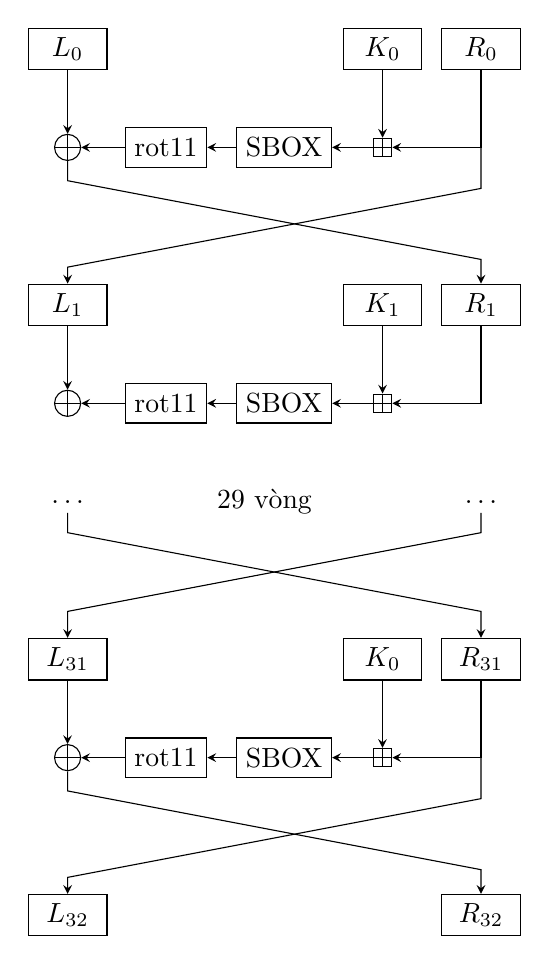
\begin{tikzpicture}[
        node distance=1.25cm
    ]
        %Round 1
        \node [block] (L0) {$L_0$};
        \node [XOR, below of=L0] (x0) {};
        \node [block, right of=x0] (s0) {$\rot$};
        \node [block, right of=s0, node distance=1.5cm] (sb0) {$\SBOX$};
        \node [BXOR, right of=sb0] (b0) {};
        \node [right of=b0] (e0) {};
        \node [block, above of=e0] (R0) {$R_0$};
        \node [block, above of=b0] (K0) {$K_0$};
        %Round 2
        \node [block, below of=x0, node distance=2cm] (L1) {$L_1$};
        \node [XOR, below of=L1] (x1) {};
        \node [block, right of=x1] (s1) {$\rot$};
        \node [block, right of=s1, node distance=1.5cm] (sb1) {$\SBOX$};
        \node [BXOR, right of=sb1] (b1) {};
        \node [right of=b1] (e1) {};
        \node [block, above of=e1] (R1) {$R_1$};
        \node [block, above of=b1] (K1) {$K_1$};
        %temp
        \node [below of=x1] (Lt) {$\ldots$};
        \node [below of=e1] (Rt) {$\ldots$};
        \node [right of=Lt, node distance=2.5cm] (txt) {29 vòng};
        %Round i
        \node [block, below of=Lt, node distance=2cm] (Li) {$L_{31}$};
        \node [XOR, below of=Li] (xi) {};
        \node [block, right of=xi] (si) {$\rot$};
        \node [block, right of=si, node distance=1.5cm] (sbi) {$\SBOX$};
        \node [BXOR, right of=sbi] (bi) {};
        \node [right of=bi] (ei) {};
        \node [block, above of=ei] (Ri) {$R_{31}$};
        \node [block, above of=bi] (Ki) {$K_0$};
        %Ciphertext
        \node [block, below of=xi, node distance=2cm] (L) {$L_{32}$};
        \node [block, below of=ei, node distance=2cm] (R) {$R_{32}$};

        \draw [-stealth] (L0) -- (x0);
        \draw [stealth-] (x0) -- (s0);
        \draw [stealth-] (s0) -- (sb0);
        \draw [stealth-] (sb0) -- (b0);
        \draw [-stealth] (K0) -- (b0);
        \draw [-stealth] (R0) |- (b0);
        \draw [-stealth] (R0.south) -- ++(0, -1.5) 
                -- ++(-5.25, -1) -| (L1.north);
        \draw [-stealth] (x0.south) -- ++(0, -0.25)
                -- ++(5.25, -1) -| (R1.north);

        \draw [-stealth] (L1) -- (x1);
        \draw [stealth-] (x1) -- (s1);
        \draw [stealth-] (s1) -- (sb1);
        \draw [stealth-] (sb1) -- (b1);
        \draw [-stealth] (K1) -- (b1);
        \draw [-stealth] (R1) |- (b1);
        
        \draw [-stealth] (Li) -- (xi);
        \draw [stealth-] (xi) -- (si);
        \draw [stealth-] (si) -- (sbi);
        \draw [stealth-] (sbi) -- (bi);
        \draw [-stealth] (Ki) -- (bi);
        \draw [-stealth] (Ri) |- (bi);
        \draw [-stealth] (Lt.south) -- ++(0, -0.25)
                -- ++(5.25, -1) -| (Ri.north);
        \draw [-stealth] (Rt.south) -- ++(0, -0.25)
               -- ++(-5.25, -1) -| (Li.north);

        \draw [-stealth] (xi.south) -- ++(0, -0.25)
               -- ++(5.25, -1) -| (R.north);
       \draw [-stealth] (Ri.south) -- ++(0, -1.5)
              -- ++(-5.25, -1) -| (L.north);
    \end{tikzpicture}
\end{document}